\newpage
\[ \text{min } Z = x_1 - 2x_2 \quad \Longrightarrow \quad \text{max } -Z = - x_1 + 2x_2 \]  

\[    
\left\{
    \begin{array}{l}
        6x_{1} + 3x_{2} \leq 18 \\[2pt]
        2x_{1} + 3x_{2} \leq 9 \\[2pt]
        x_{1}, x_{2} \text{ are integers}
    \end{array}
    \right.
\]

\begin{center}
    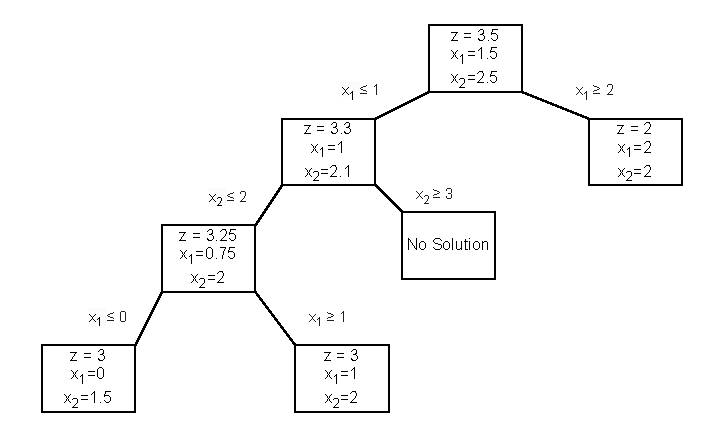
\includegraphics{Exercice/PY/EX2/b2.drawio.pdf}
\end{center}

\vspace{0.5cm}

\[\text{Optimal Solution is }\hspace{0.1cm} \boxed{(x_1,x_2) = (1,2)}\]


\vspace{0.5cm}

\begin{prettyBox}{Note}{red}
We did not branch the node (\(Z = 3, x_1 = 0, x_2 = 1.5\)) because another node 
at the same level (\(Z = 3, x_1 = 1, x_2 = 2\)) was already completed. Continuing 
to branch the first node would only cause \(Z\) to keep decreasing. Hence, we pruned it.
\end{prettyBox}

\begin{center}
    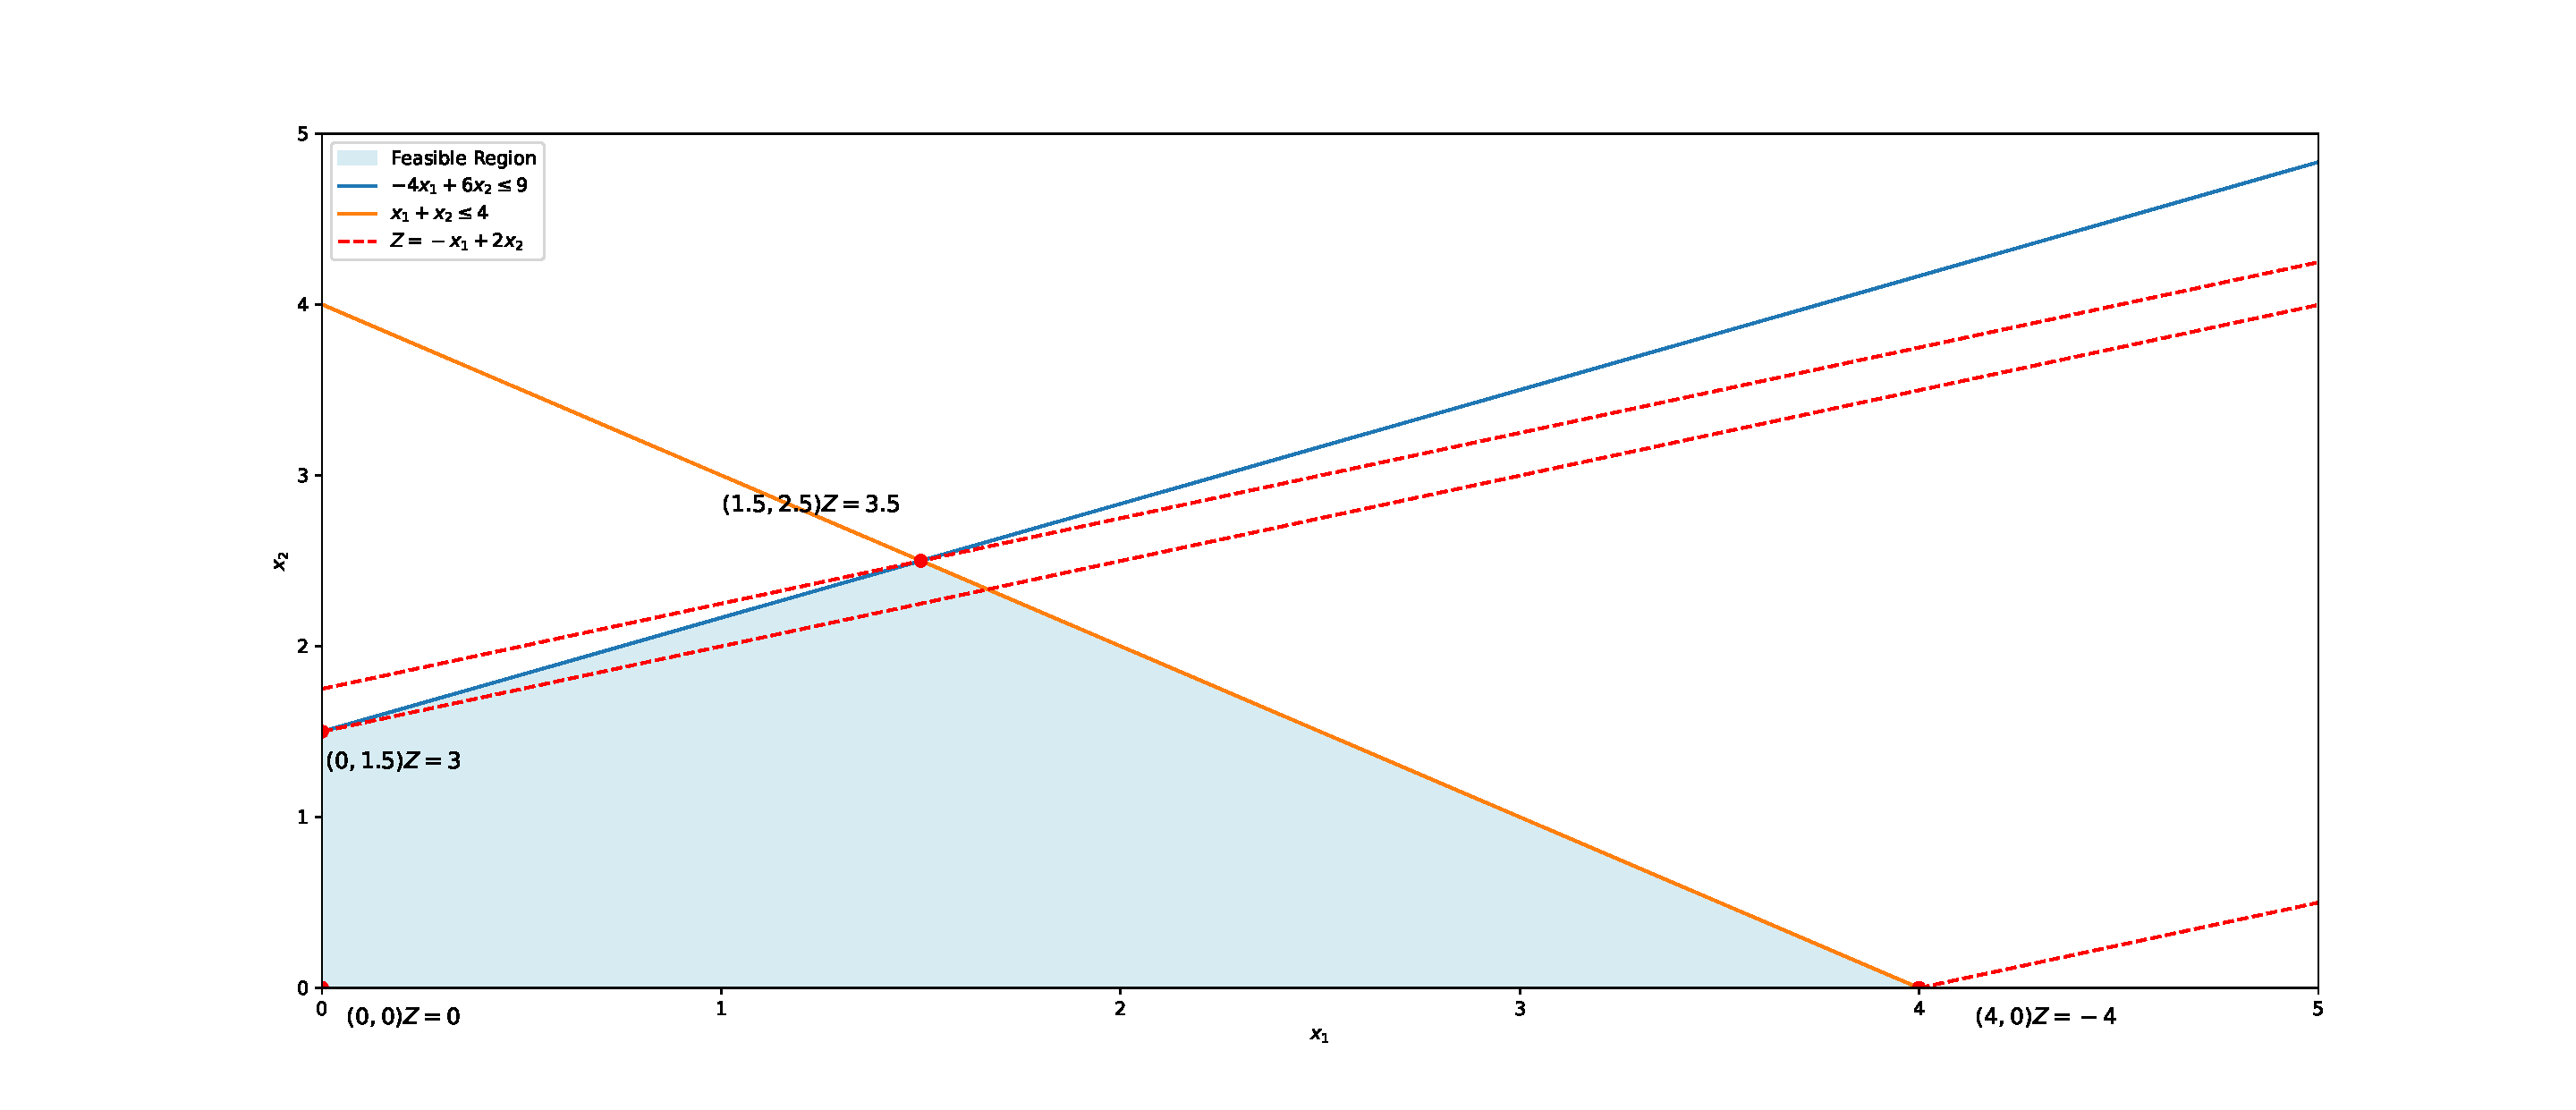
\includegraphics[width = \textwidth]{Exercice/PY/EX2/ex2.1.pdf}
\end{center}


\begin{center}
    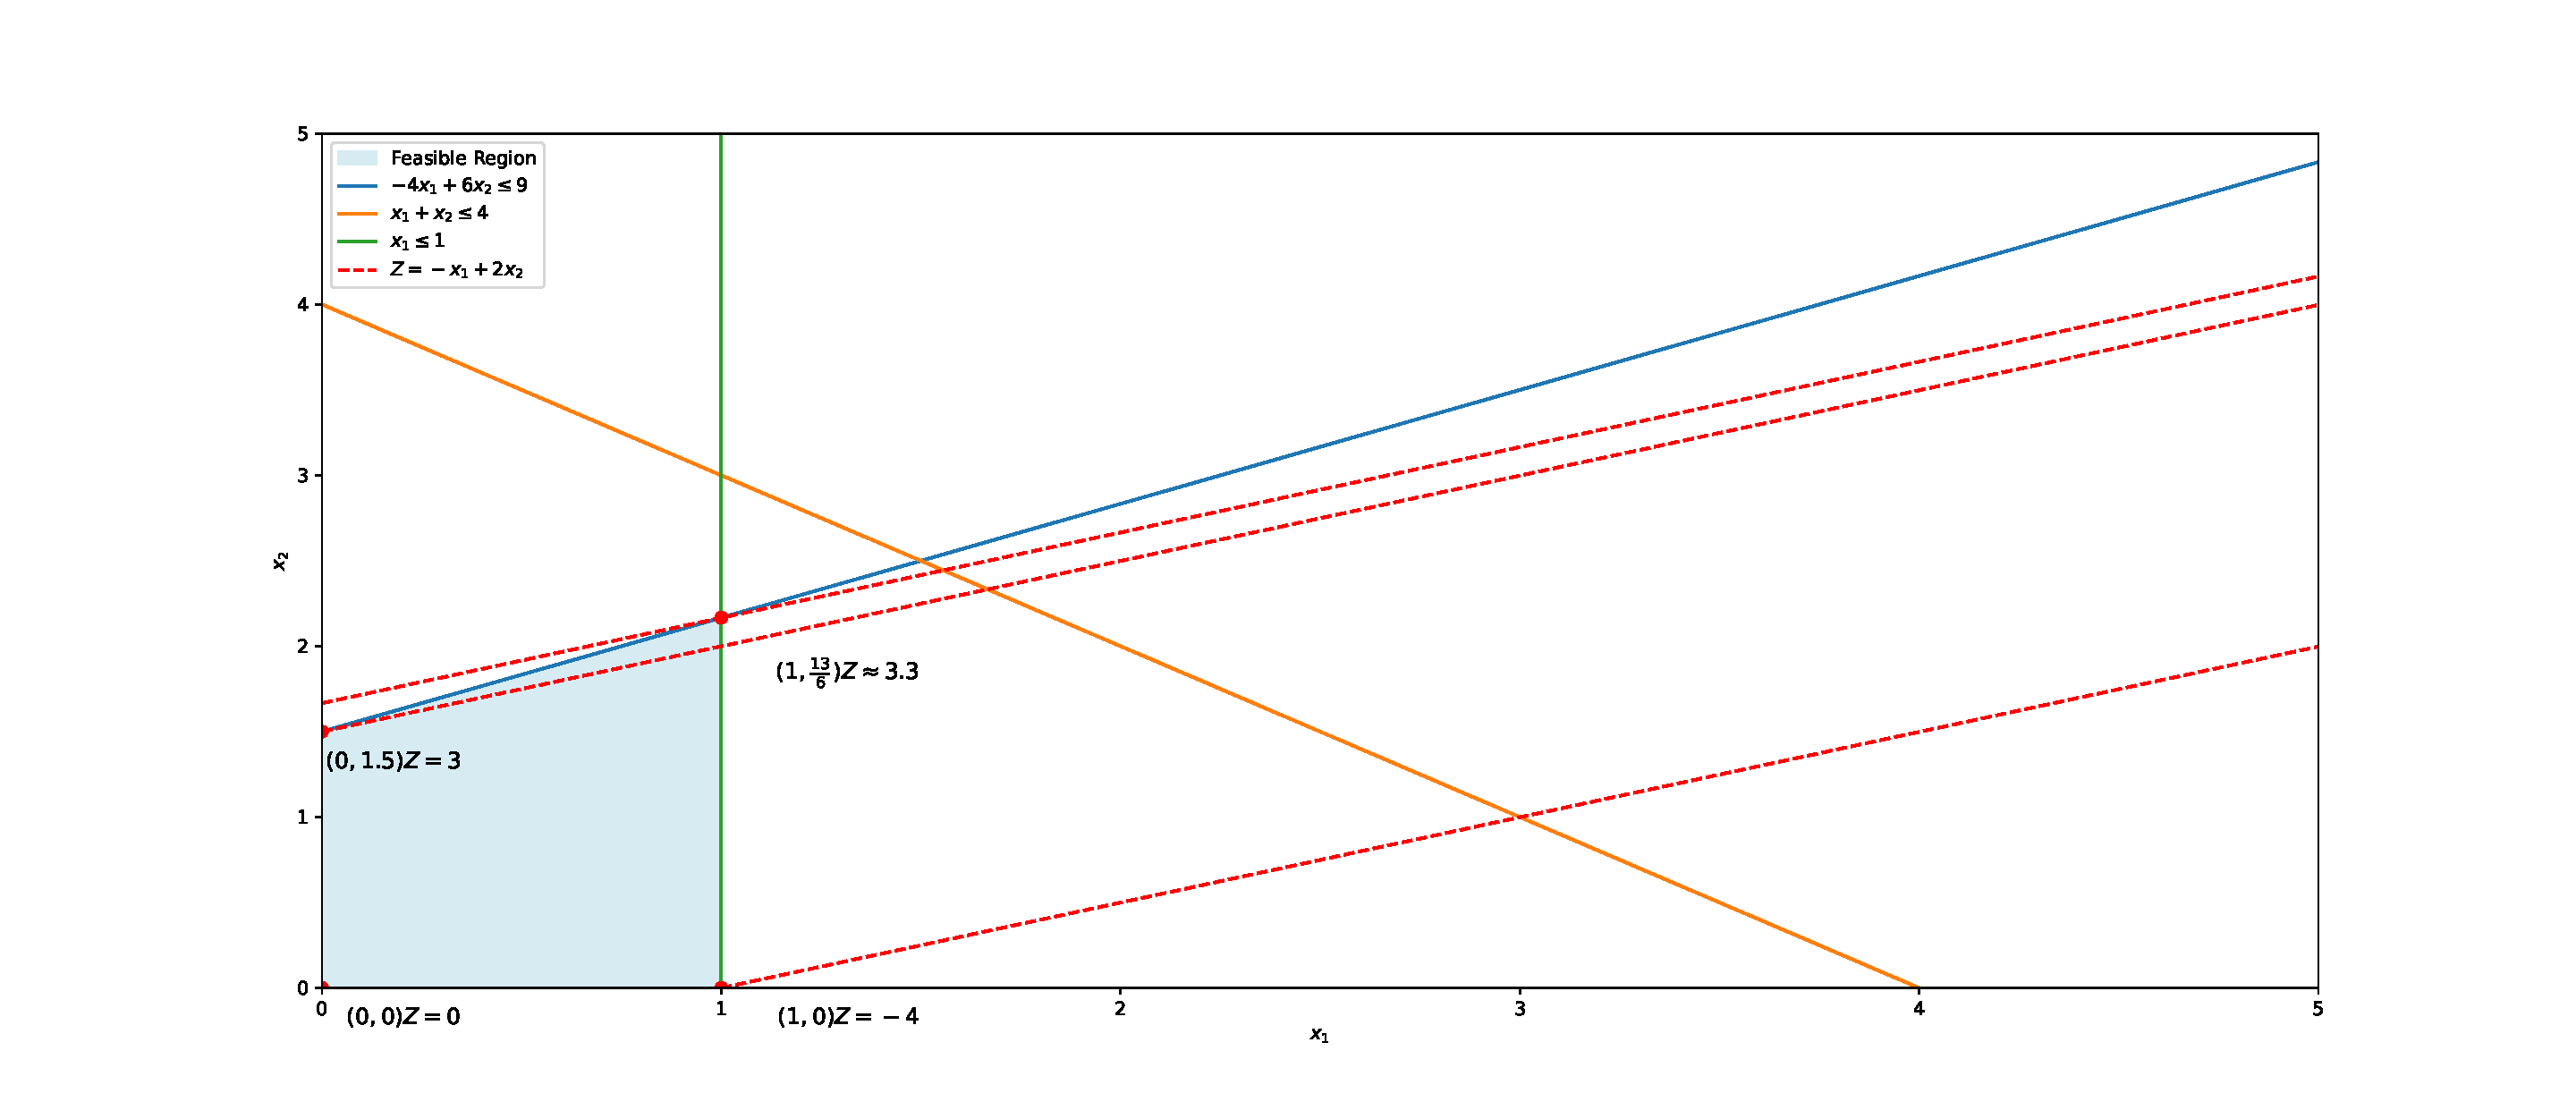
\includegraphics[width = \textwidth]{Exercice/PY/EX2/ex2.2.pdf}
\end{center}


\begin{center}
    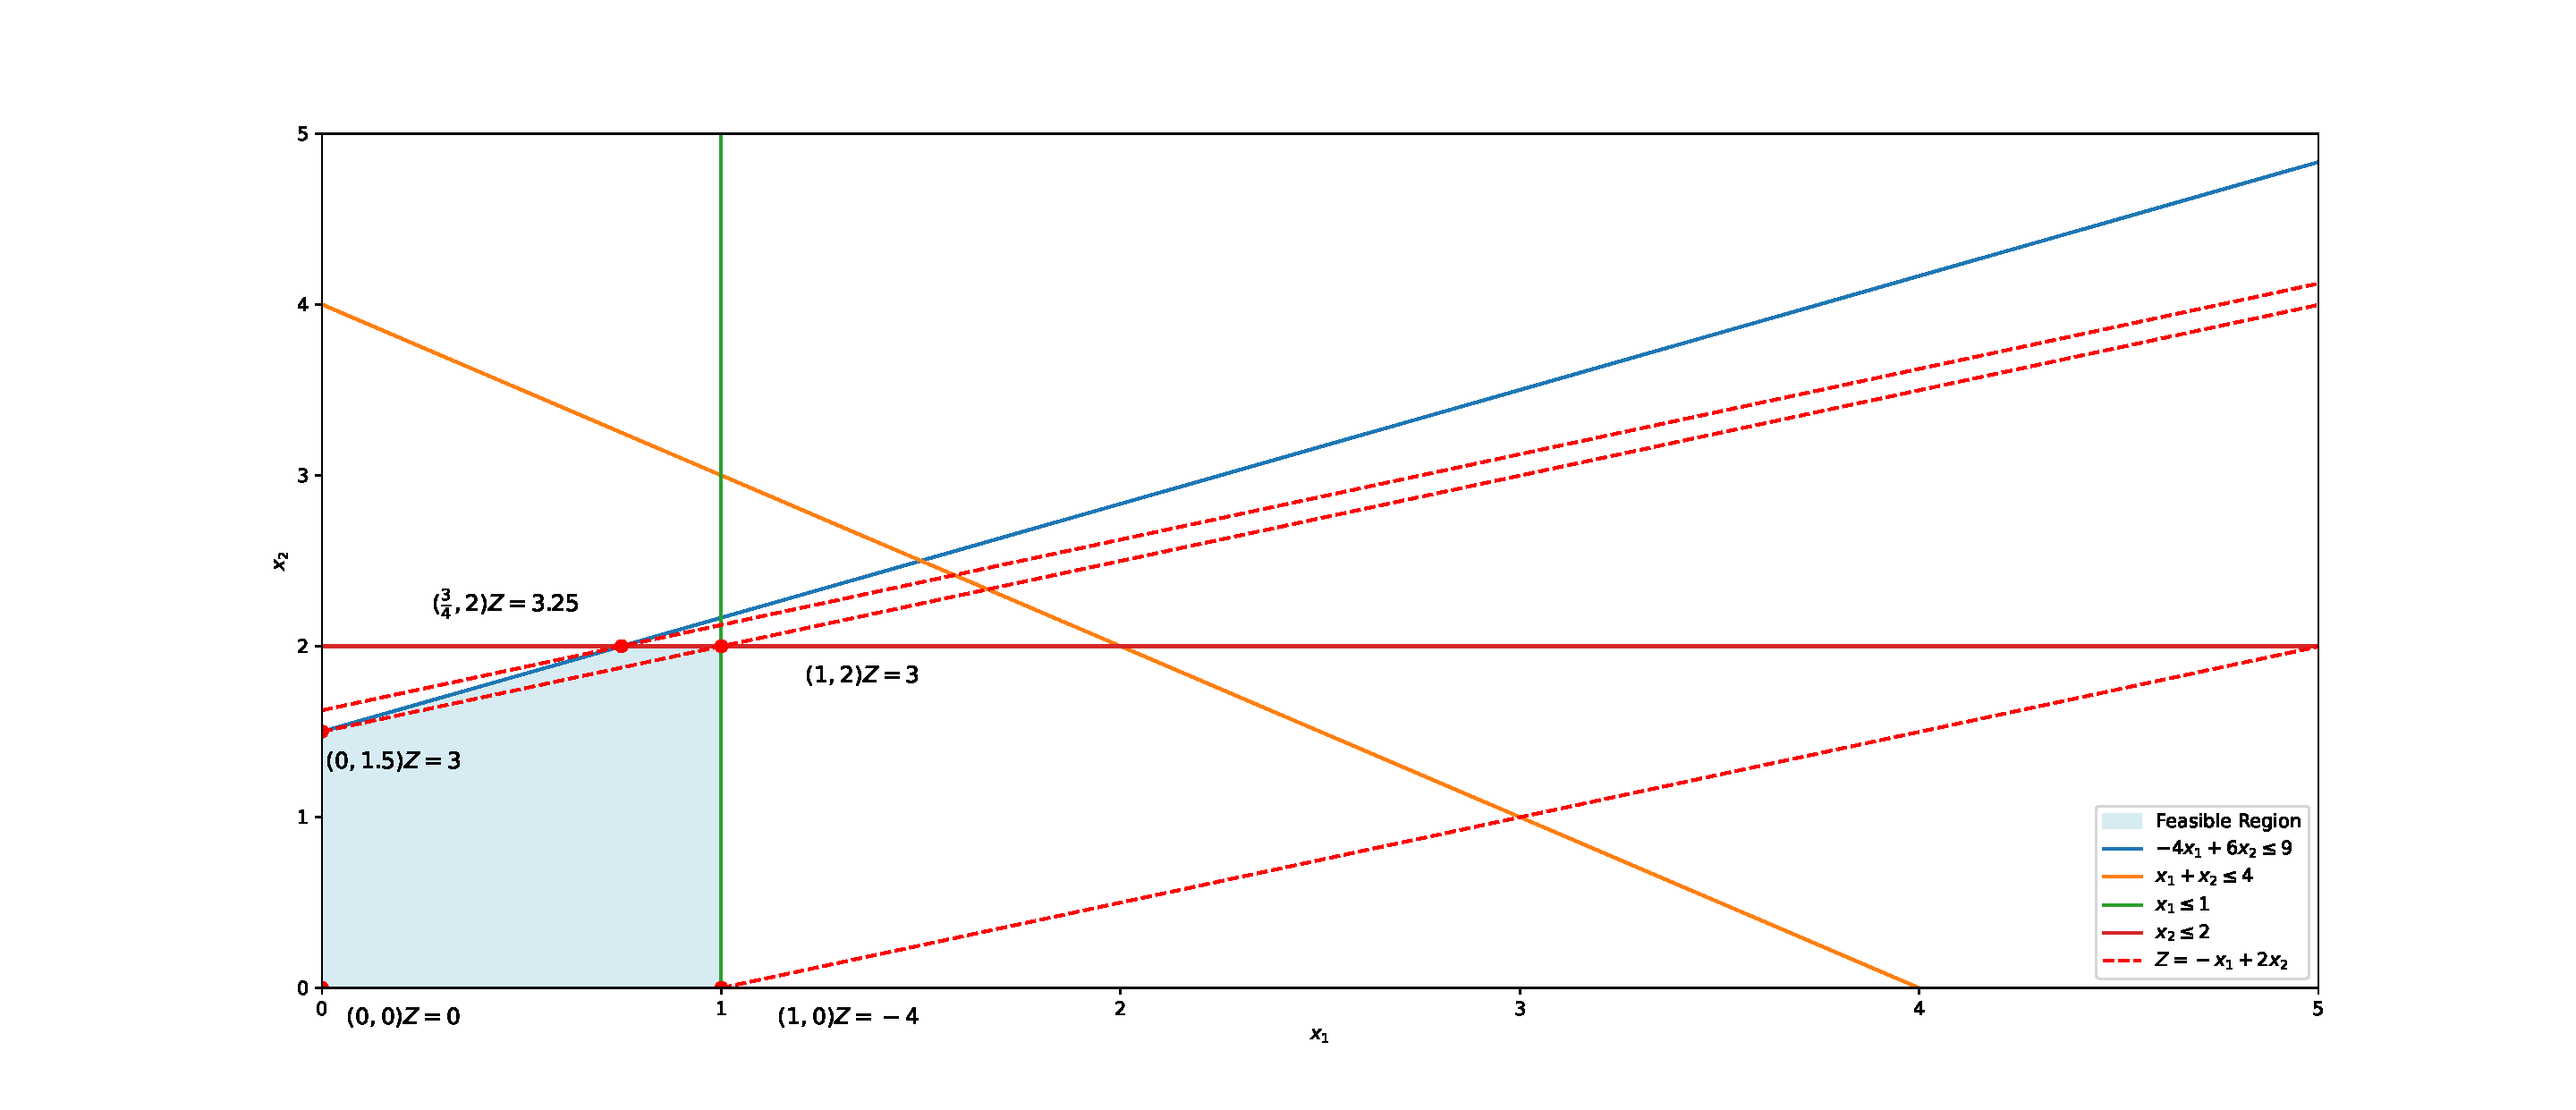
\includegraphics[width = \textwidth]{Exercice/PY/EX2/ex2.3.pdf}
\end{center}

\begin{center}
    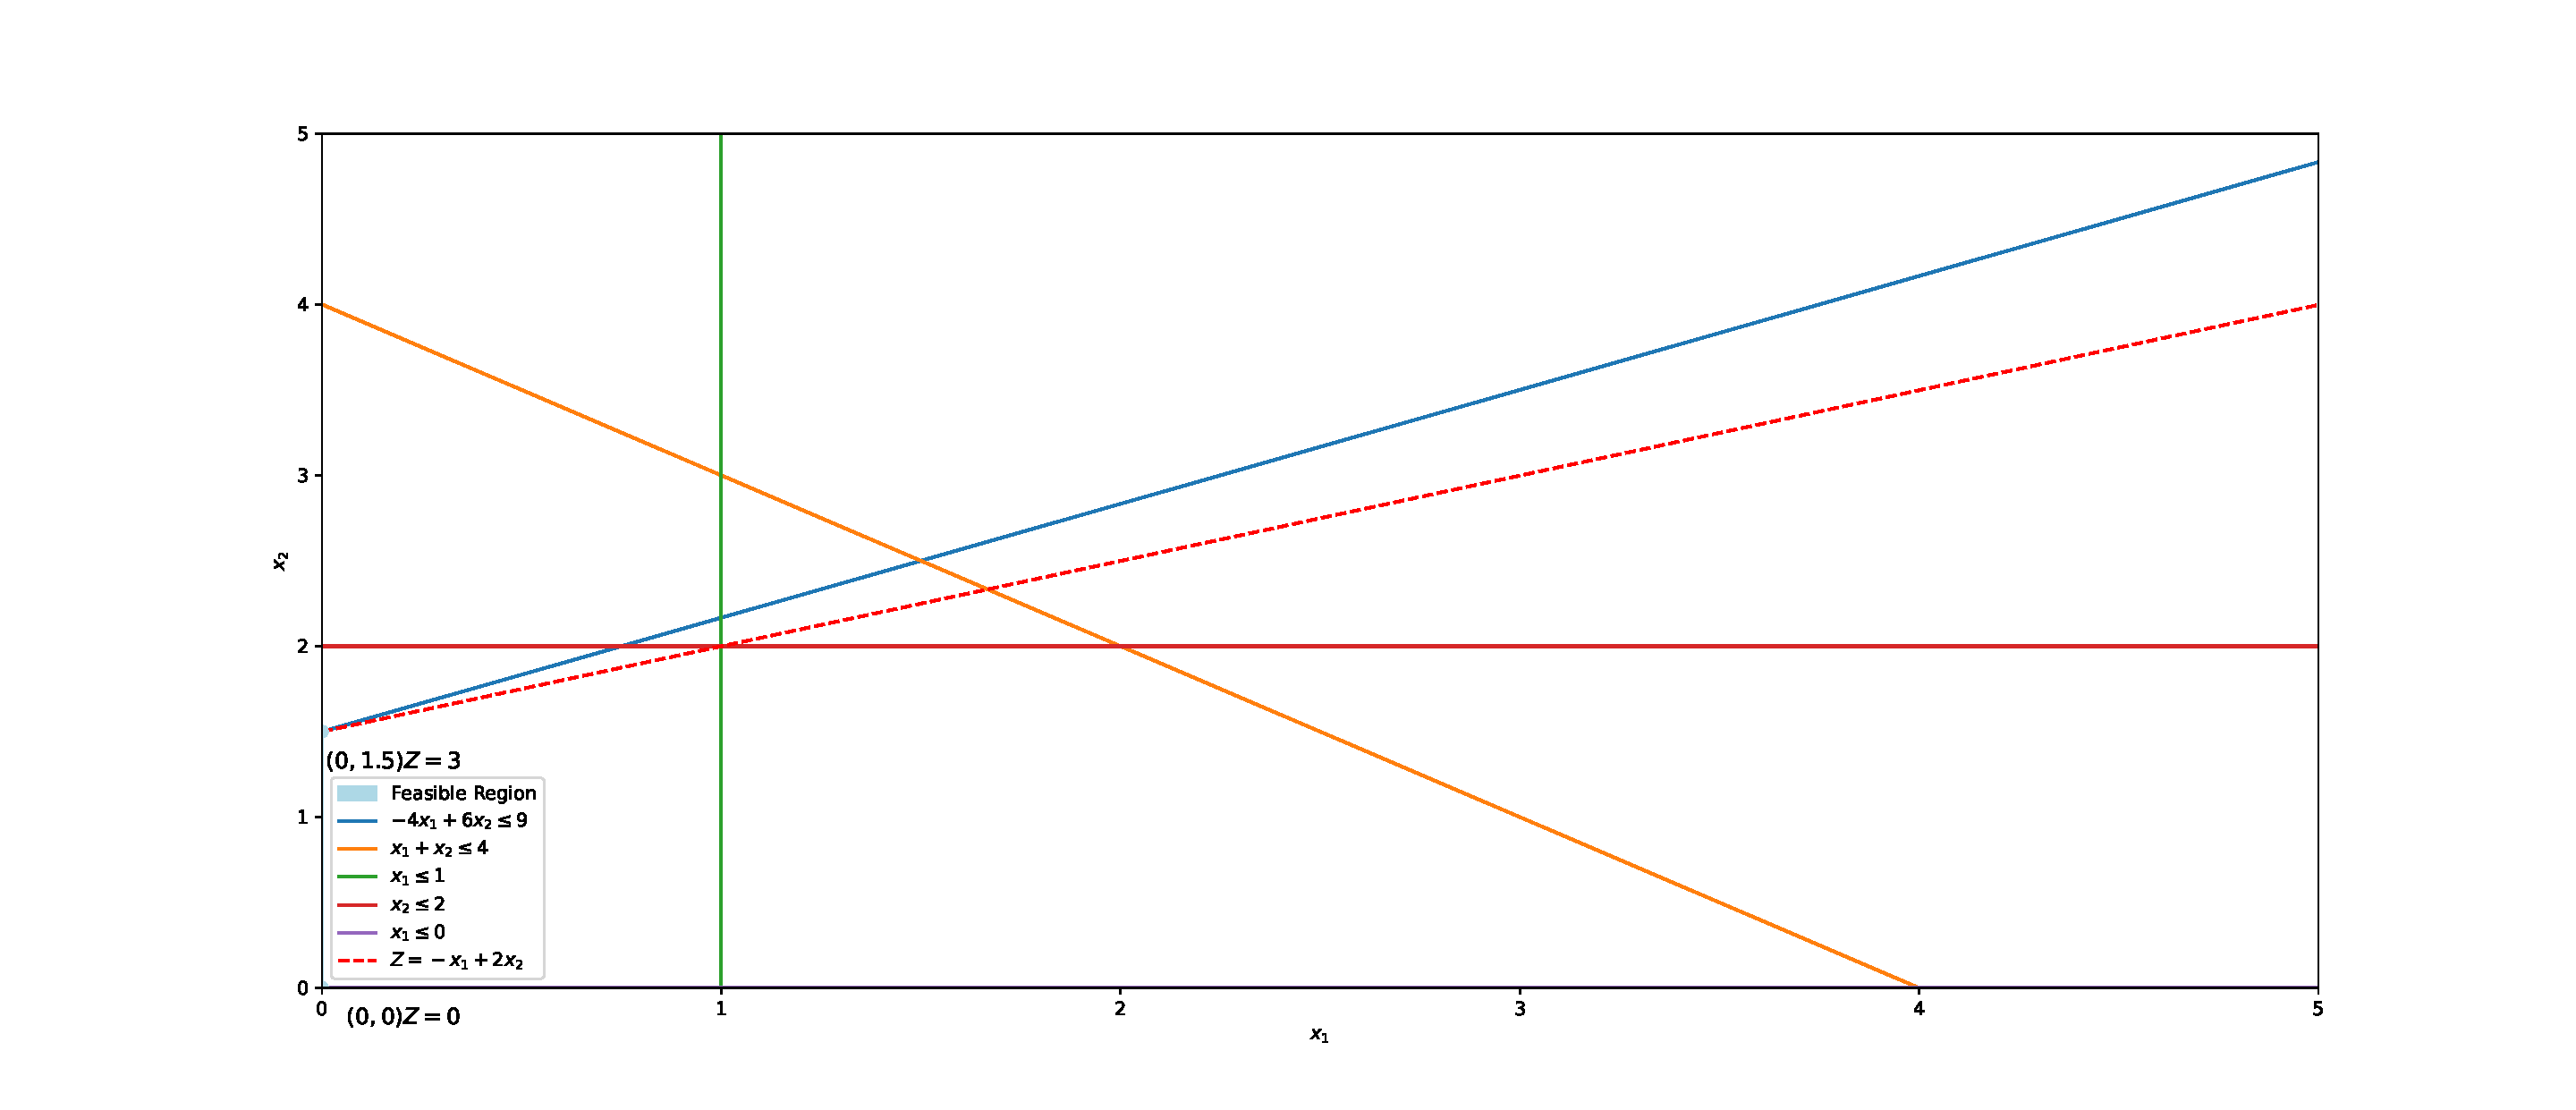
\includegraphics[width = \textwidth]{Exercice/PY/EX2/ex2.4.pdf}
\end{center}
\begin{center}
    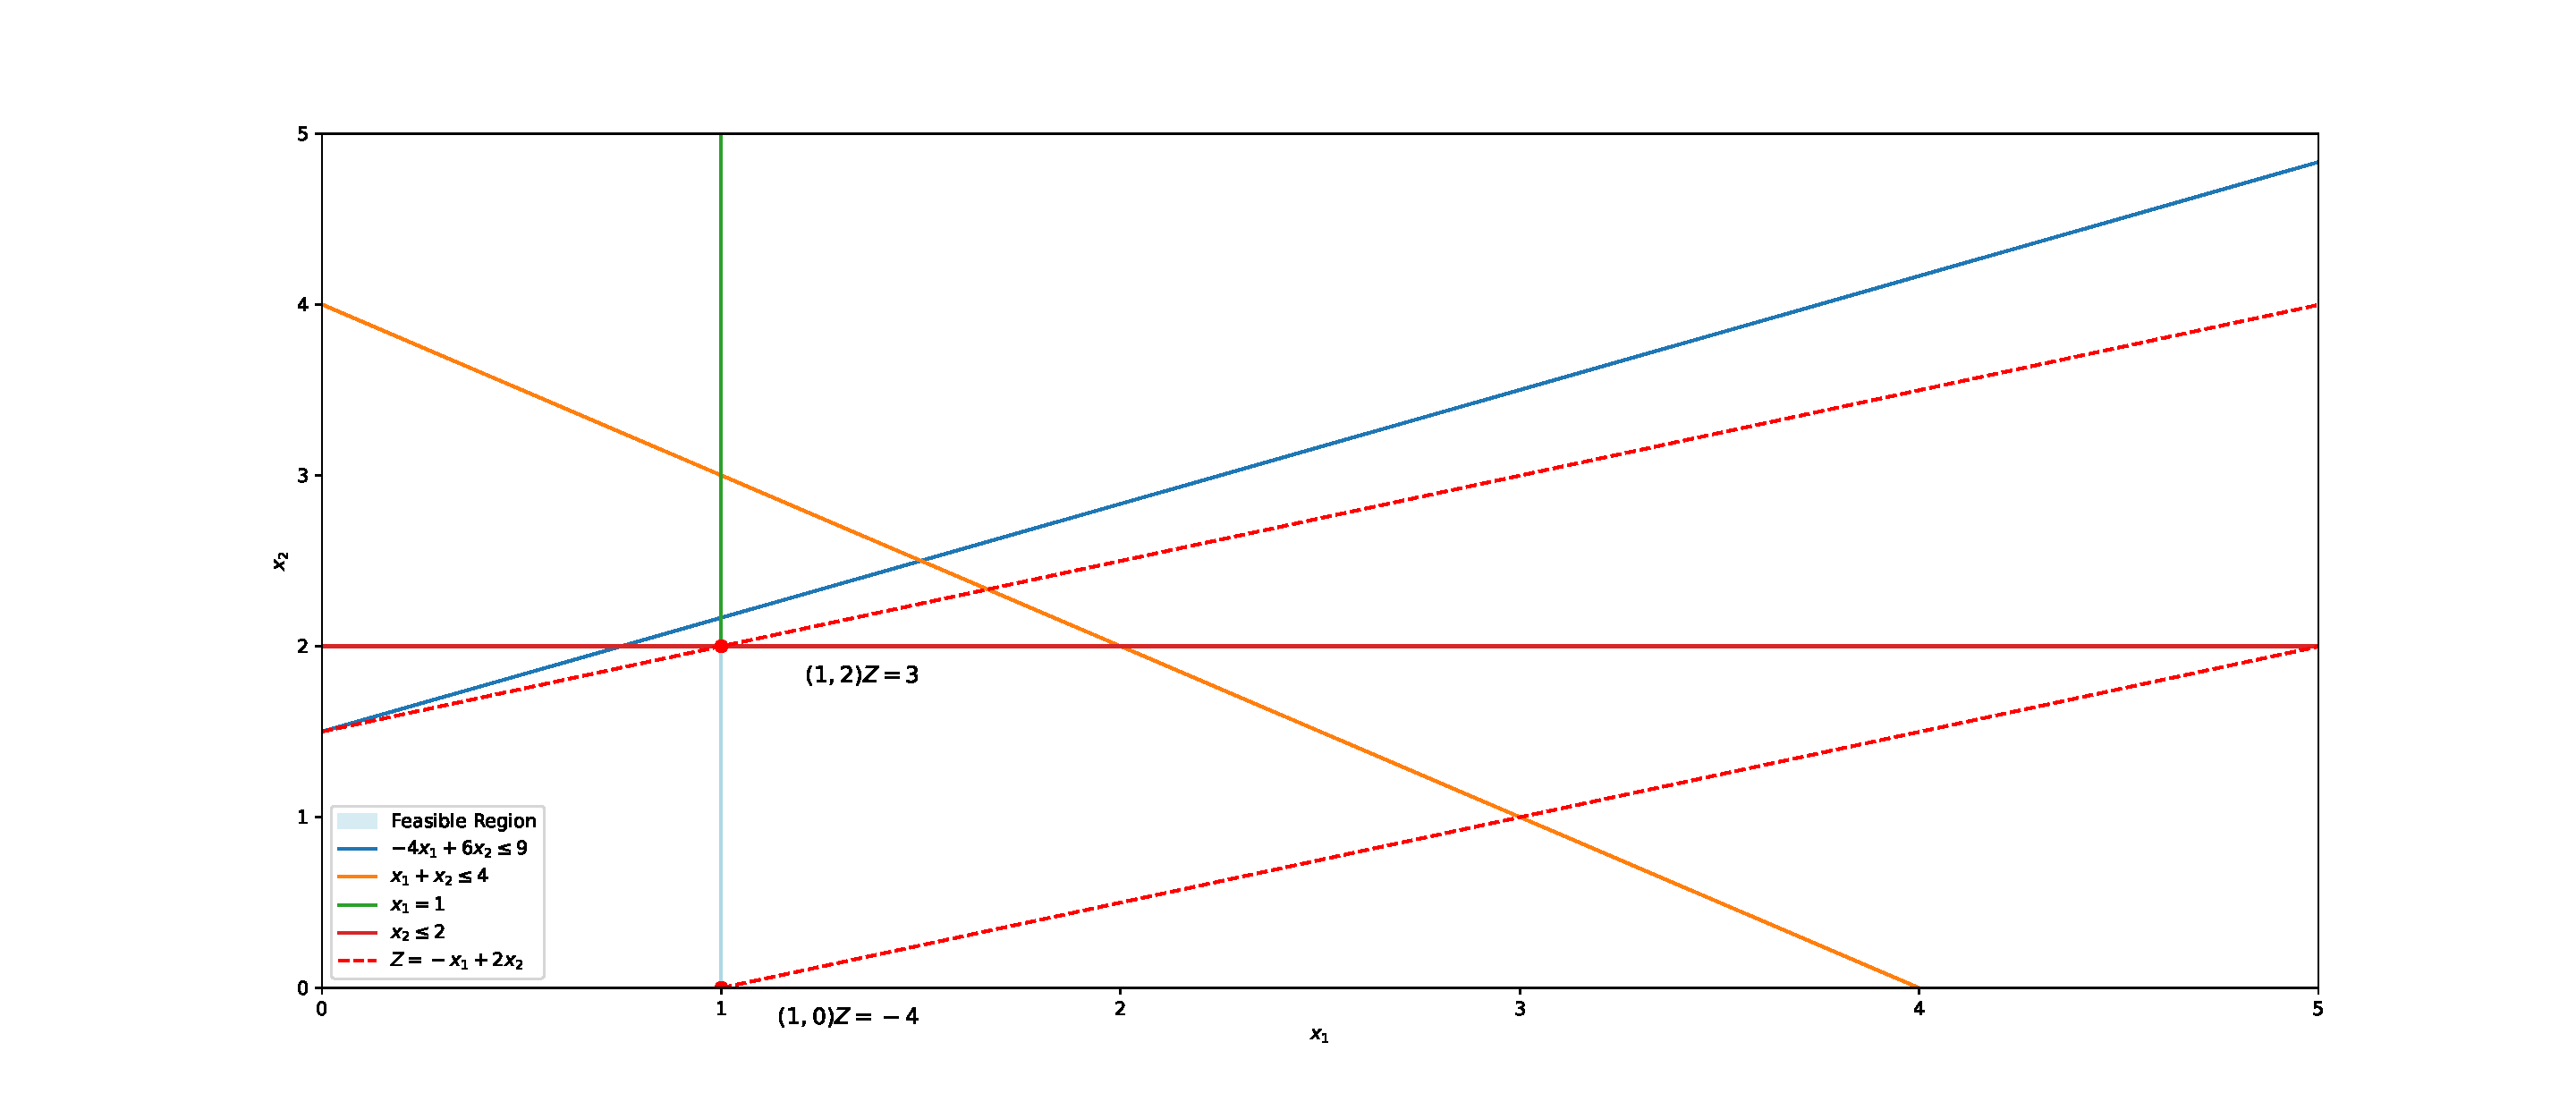
\includegraphics[width = \textwidth]{Exercice/PY/EX2/ex2.5.pdf}
\end{center}
\begin{center}
    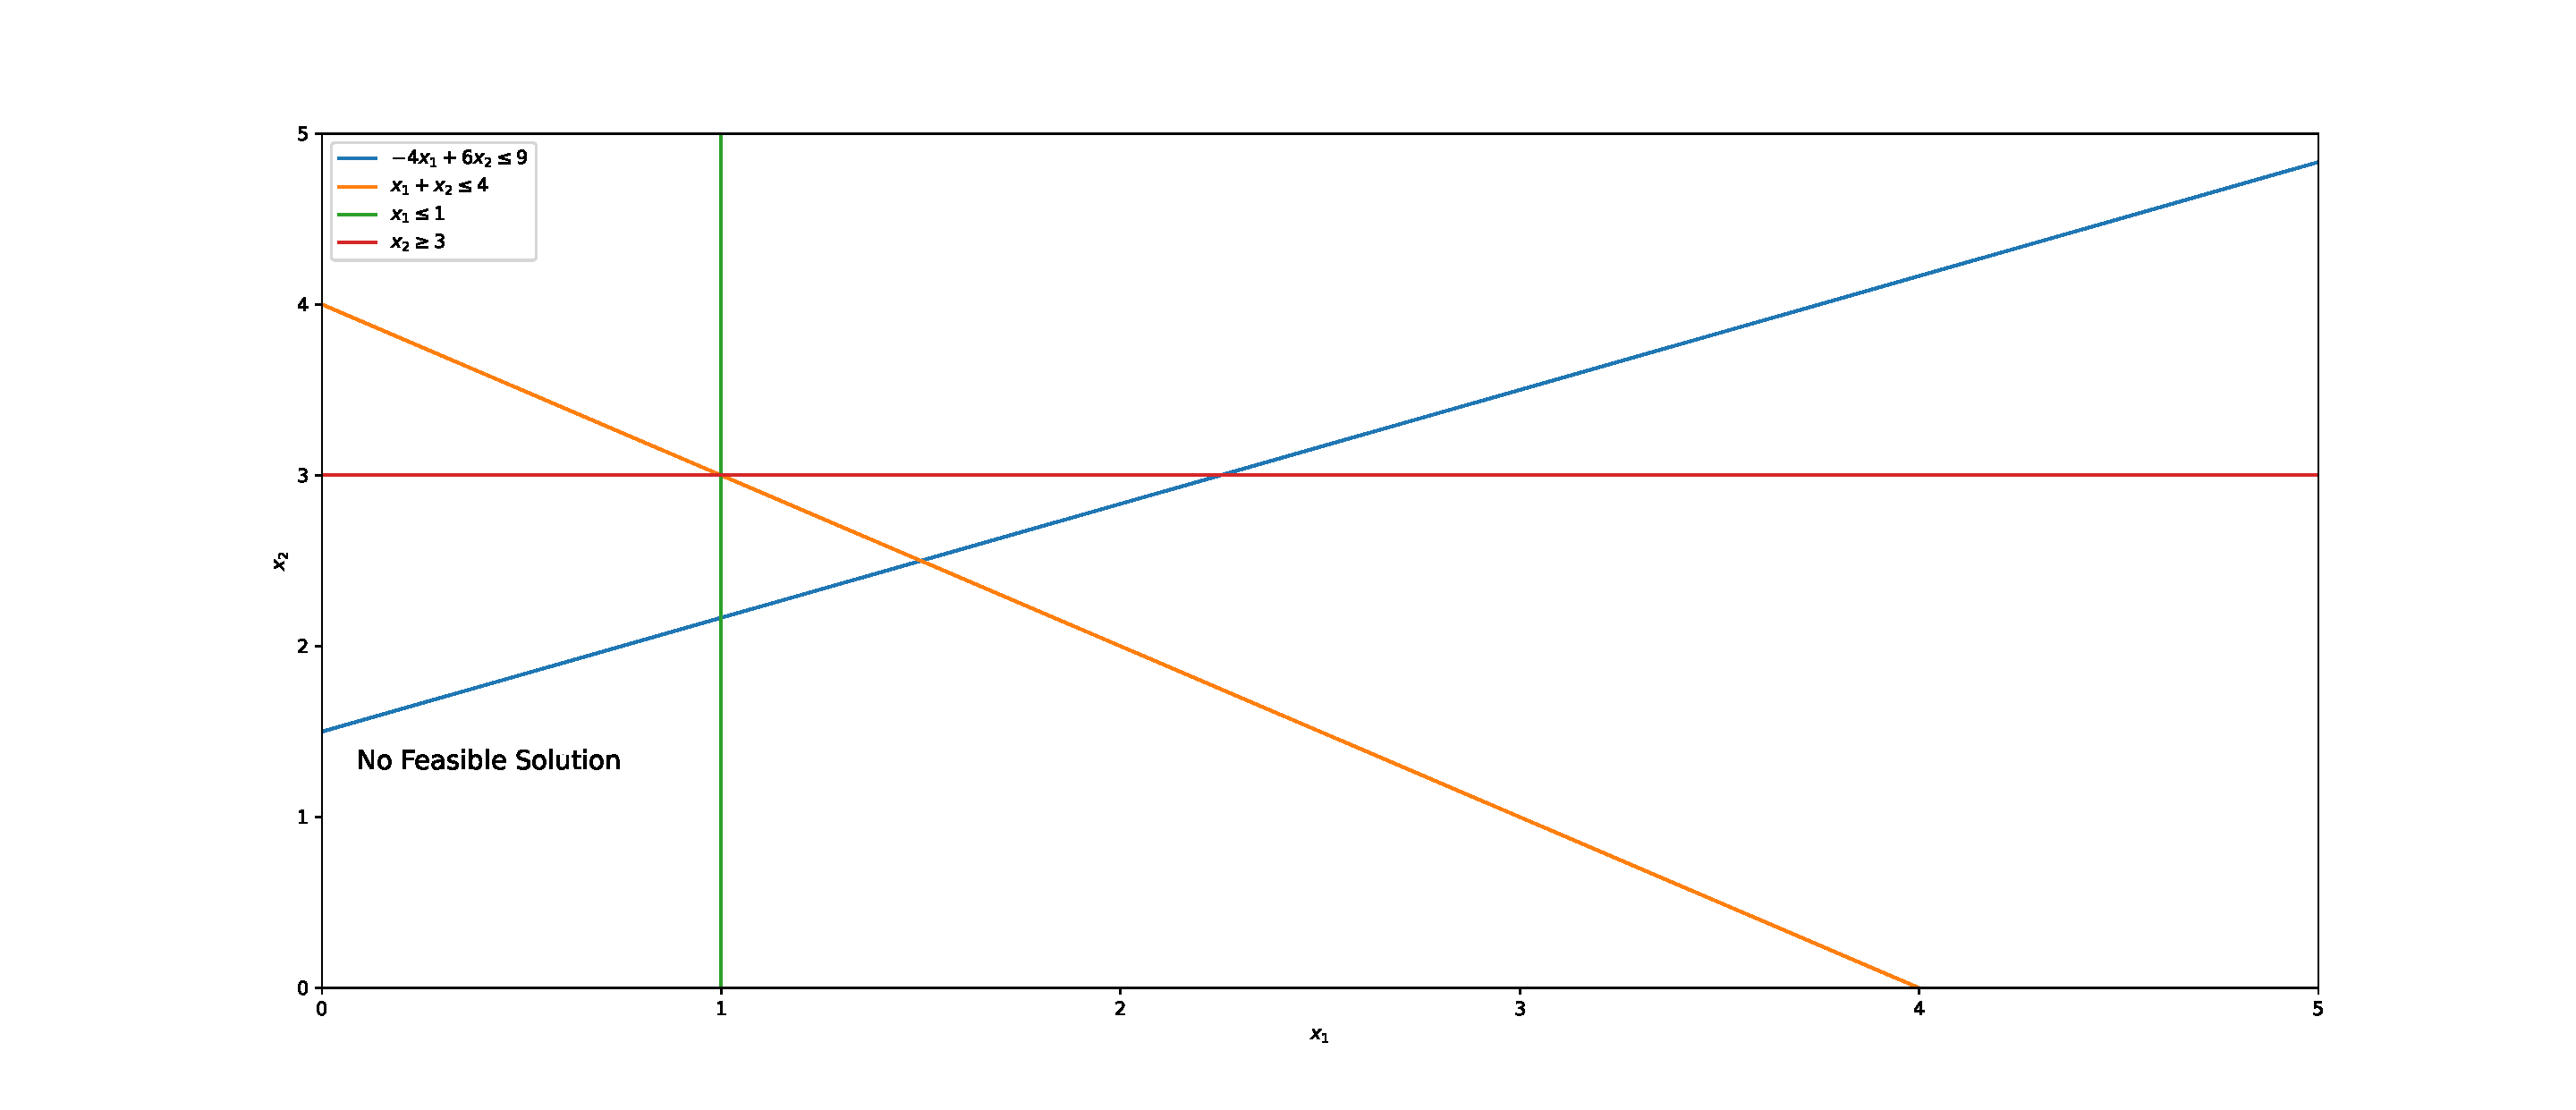
\includegraphics[width = \textwidth]{Exercice/PY/EX2/ex2.6.pdf}
\end{center}
\begin{center}
    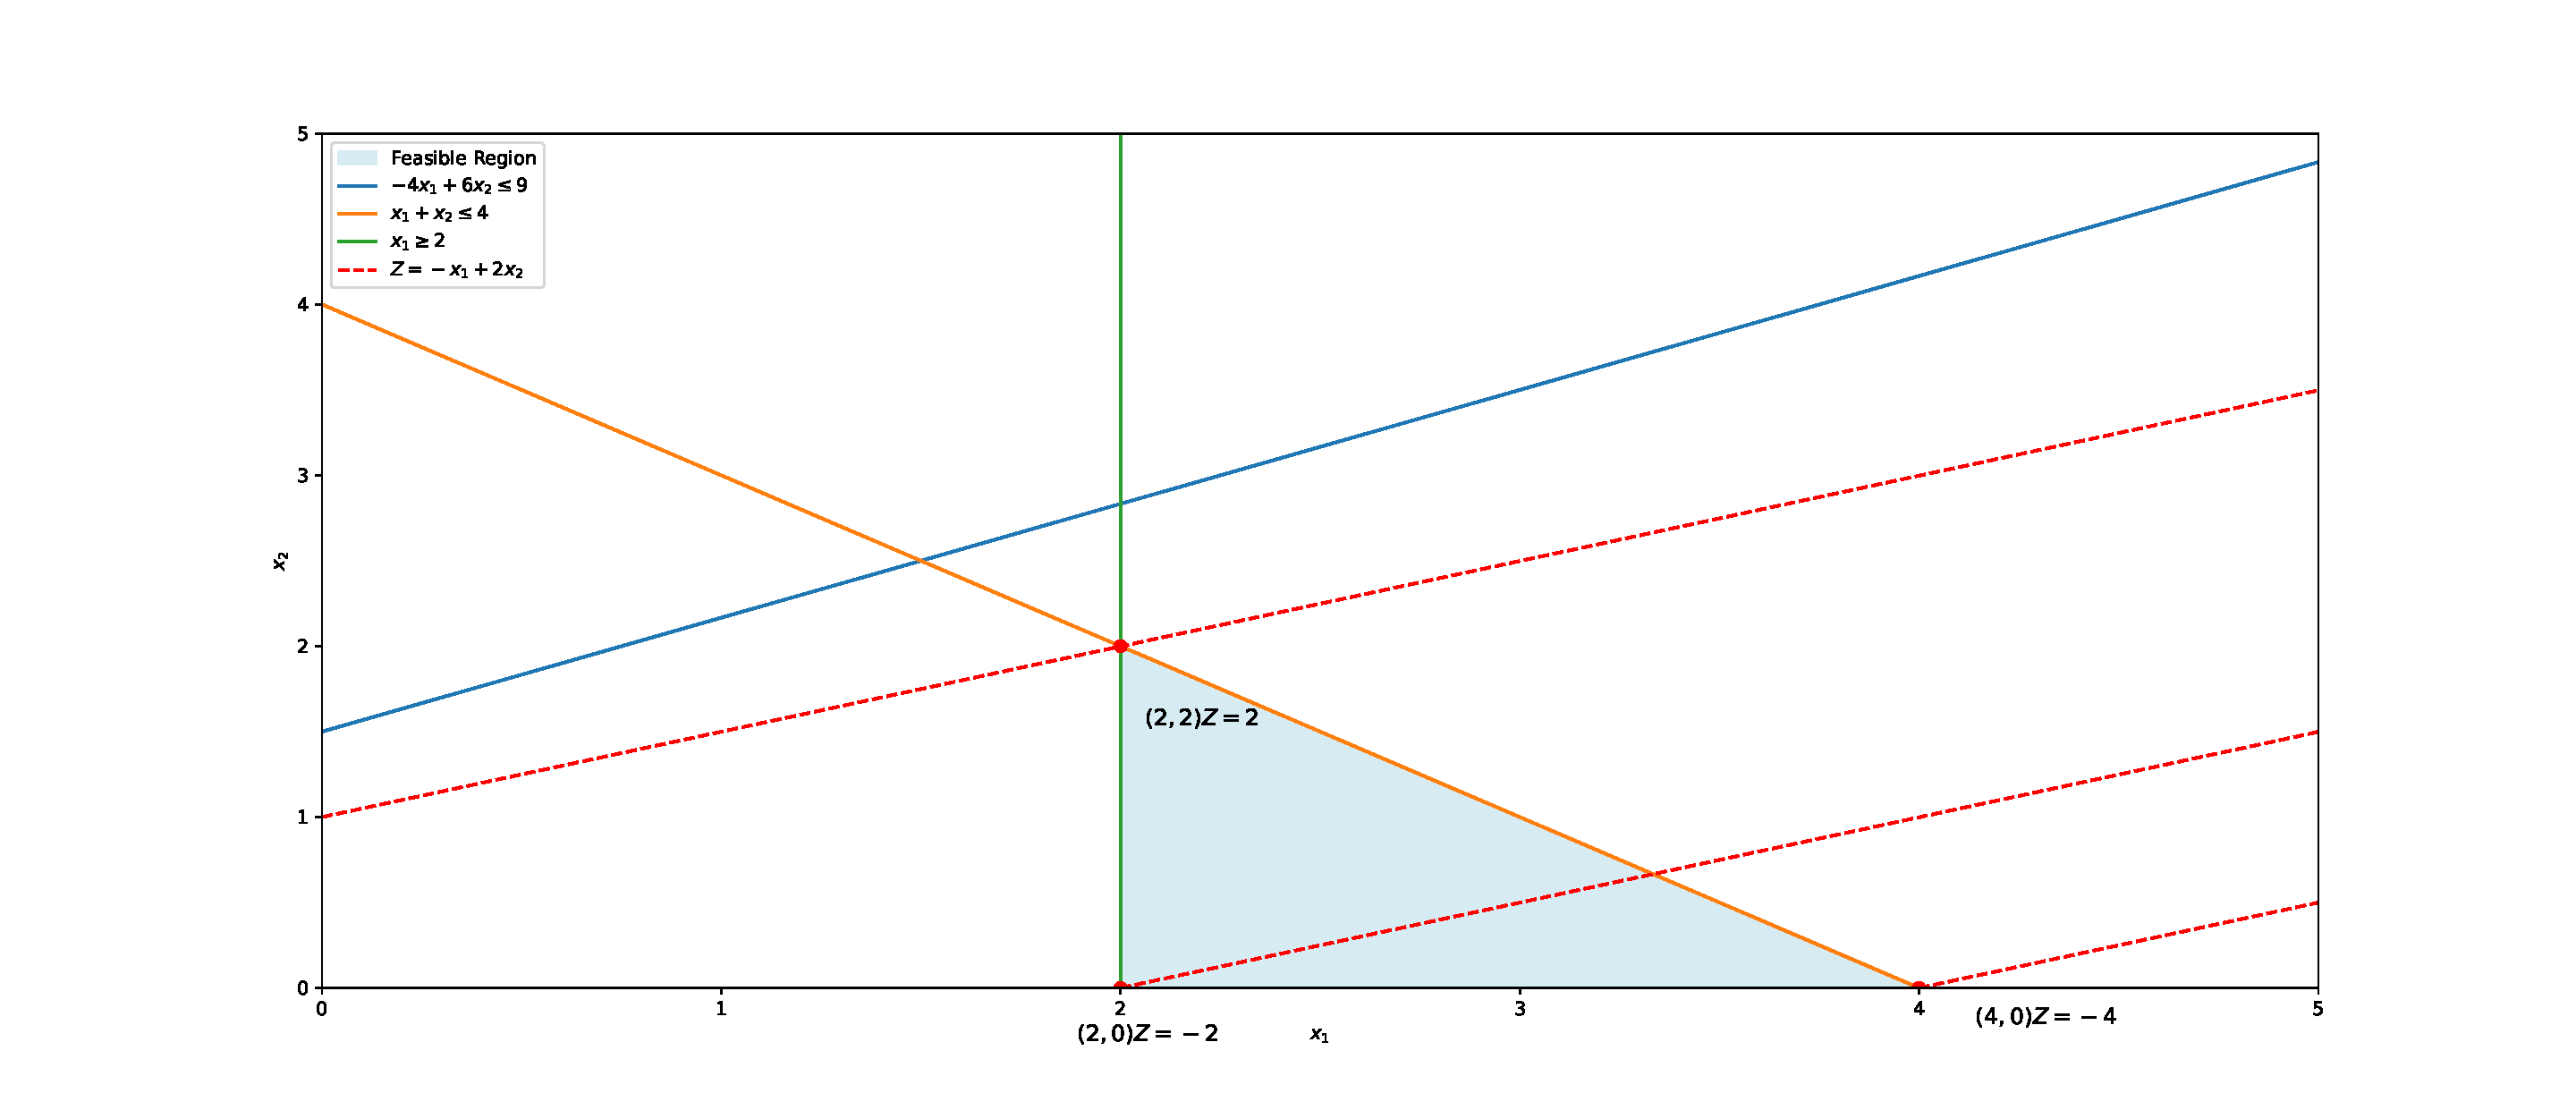
\includegraphics[width = \textwidth]{Exercice/PY/EX2/ex2.7.pdf}
\end{center}

